\documentclass[5]{article}
\usepackage[utf8]{inputenc}
\usepackage{hyperref} 

\usepackage[T1]{fontenc}
\usepackage[polish]{babel}

\title{Laboratorium 2}
\author{Piotr Witek}
\date{17 marca 2021}

\usepackage{natbib}
\usepackage{graphicx}
\usepackage{geometry}
\usepackage{tabularx}
\usepackage{array}
\usepackage{amsmath}

\begin{document}

\newgeometry{tmargin=2cm, bmargin=2cm, lmargin=2.5cm, rmargin=2.5cm}

\maketitle

\section{Zadania}

\subsection{Dane są trzy węzły interpolacji (-2.9,1), (0,1.5), (2.3,3.9), proszę obliczyć wielomian interpolacyjny 2-go stopnia, wykorzystując:}

\subsubsection{jednomiany}

Bazę stanowią funkcje 1, x, $x^2$. Funkcja interpulująca będzie mieć postać:

\[w(x) = ax^2+bx+c\]

\begin{flushleft}
Wyznaczam i rozwiązuję układ równań:
\end{flushleft}

\begin{flushleft}
$
\left\{ \begin{array}{ll}
w(-2.9)=1\\
w(0)=1.5\\
w(2.3) = 3.9
\end{array} \right.
$
\end{flushleft}
\begin{flushleft}
$
\left\{ \begin{array}{ll}
8.41a-2.9b+c=1\\
c=1.5\\
5.29+2.3b+c=3.9
\end{array} \right.
$
\end{flushleft}

\begin{flushleft}
$
\left\{
\arraycolsep=1.4pt\def\arraystretch{1.5}
\begin{array}{ll}
a=\frac{2905}{17342}\\
b=\frac{22829}{34684}\\
c=\frac{3}{2}
\end{array} \right.
$
\end{flushleft}

\begin{flushleft}
Zatem $w(x)=\frac{2905}{17342}x^2+\frac{22829}{34684}x+\frac{3}{2}$
\end{flushleft}

\subsubsection{wielomiany Lagrange'a}

Bazą są trzy funkcje $L_{i}$ postaci:
\[L_{i}(x)=\prod_{j=0, j\neq i}^{n}\frac{x-x_{j}}{x_{i}-x_{j}}\]

Wielomian interpolacyjny ma postać:
\[w(x)=\sum_{i=0}^{n}f_{i}\cdot L_{i}(x)\]

gdzie $f_{i}$ to wartość wielomianu interpolowanego w i-tym węźle interpolacji. Zatem:

\[w(x)=1\cdot \frac{x}{-2.9}\cdot \frac{x-2.3}{-2.9-2.3}+1.5\cdot \frac{x+2.9}{2.9}\cdot \frac{x-2.3}{-2.3}+3.9\cdot \frac{x+2.9}{2.3+2.9}\cdot \frac{x}{2.3}\]

\[w(x)=\frac{2905}{17342}x^2+\frac{22829}{34684}x+\frac{3}{2}\]

\subsubsection{wielomiany wg wzoru Newtona}

Wielomian interpolujący ma postać:

\[w(x)=\sum_{i=0}^{n}a_{i}\prod_{j=0}^{i-1}(x-x_{j})\]
\[w(x)=a_{0}+a_{1}(x-x_{0})+a_{2}(x-x_{0})(x-x_{1})\]
\[w(x)=a_{0}+a_{1}(x+2.9)+a_{2}x(x+2.9)\]

\begin{flushleft}
Wyznaczam i rozwiązuję układ równań:
\end{flushleft}

\begin{flushleft}
$
\left\{ \begin{array}{ll}
w(-2.9)=a_{0}+a_{1}(-2.9+2.9)+a_{2}(-2.9)(-2.9+2.9)=1\\
w(0)=a_{0}+a_{1}(0+2.9)+a_{2}\cdot 0 \cdot(0+2.9)=1.5\\
w(2.3)=a_{0}+a_{1}(2.3+2.9)+a_{2}\cdot 2.3 \cdot(2.3+2.9)=3.9
\end{array} \right.
$
\end{flushleft}

\begin{flushleft}
$
\left\{
\arraycolsep=1.4pt\def\arraystretch{1.5}
\begin{array}{ll}
a_{0}=1\\
a_{1}=\frac{5}{29}\\
a_{2}=\frac{2905}{17342}
\end{array} \right.
$
\end{flushleft}

Zatem wielomian interpolacyjny ma postać:
\[w(x)=\frac{2905}{17342}x^2+\frac{22829}{34684}x+\frac{3}{2}\]

Każda z metod daje tożsamy wynik postaci wielomianu interpolacyjnego.

\subsection{Wyrazić następujący wielomian metodą Hornera: $p(t) = 3t^{3}-7t^{2}+5t-4$}
\[p(t) = 3t^{3}-7t^{2}+5t-4 = t\cdot (3t^{2}-7t+5)-4 = t\cdot(t\cdot (3t-7)+5)-4 \]

\subsection{Ile mnożeń trzeba wykonać do ewaluacji  wielomianu p(t) stopnia n-1 w danym punkcie t jeżeli wybieramy jako reprezentacje:}

\subsubsection{jednomiany}
Wielomian stopnia n-1 ma postać:
\[w(x)=a_{0}+a_{1}x+...+a_{n-1}x^{n-1}\]

W takiej postaci potrzebujemy $0+1+2...+(n-1) = \frac{(n-1)\cdot n}{2}$ mnożeń.

\subsubsection{wielomiany Lagrange'a}
\[L_{i}(x)=\prod_{j=0, j\neq i}^{n-1}\frac{x-x_{j}}{x_{i}-x_{j}}\]
\[w(x)=\sum_{i=0}^{n-1}f_{i}\cdot L_{i}(x)\]

Począwszy od funkcji bazowych $L_{i}$ mamy n mnożeń prostych ilorazów, gdzie jeden iloraz to jedno mnożenie przez odwrotność, co daje 2n mnożeń.
Następnie obliczenie wartości wielomianu wymaga n-krotnego wykonania powyższych mnożeń. W rezultacie potrzeba $2n^2$ mnożeń.



\subsubsection{wielomiany Newtona}
\[w(x)=\sum_{i=0}^{n-1}a_{i}\prod_{j=0}^{i-1}(x-x_{j})\]

Mamy n składników, które wymagają kolejno 0,1,2,...,n mnożeń. Zatem łączna liczba potrzebnych mnożeń wynosi:

\[0+1+2+...+n=\frac{n(n+1)}{2}=\frac{n^2+n}{2}\]

\section{Zadania domowe}

\subsection{Obliczyć wielomian interpolacyjny dla danych (0.5,5.5), (1,14.5), (1.5,32.5), (2,62.5)}

\subsubsection{jednomiany}


Bazę stanowią funkcje 1, x, $x^2$ oraz $x^3$ . Funkcja interpulująca będzie mieć postać:

\[w(x) = ax^3+bx^2+cx+d\]

\begin{flushleft}
Wyznaczam i rozwiązuję układ równań:
\end{flushleft}

\begin{flushleft}
$
\left\{ \begin{array}{ll}
w(0.5)=5.5\\
w(1)=14.5\\
w(1.5) = 32.5\\
w(2) = 62.5
\end{array} \right.
$
\end{flushleft}
\begin{flushleft}
$
\left\{ \begin{array}{ll}
\frac{1}{8}a+\frac{1}{4}b+\frac{1}{2}c+d=\frac{11}{2}\\
a+b+c+d=\frac{29}{2}\\
\frac{27}{8}a+\frac{9}{4}b+\frac{3}{2}c+d=\frac{65}{2}\\
8a+4b+2c+d=\frac{125}{2}
\end{array} \right.
$
\end{flushleft}

\begin{flushleft}
$
\left\{ \begin{array}{ll}
a=4\\
b=6\\
c=2\\
d=2.5
\end{array} \right.
$
\end{flushleft}

\begin{flushleft}
Zatem $w(x)=4x^3+6x^2+2x+2.5$
\end{flushleft}

\subsubsection{wielomian Lagrange’a}


Bazą są cztery funkcje $L_{i}$ postaci:
\[L_{i}(x)=\prod_{j=0, j\neq i}^{n}\frac{x-x_{j}}{x_{i}-x_{j}}\]

Wielomian interpolacyjny ma postać:
\[w(x)=\sum_{i=0}^{n}f_{i}\cdot L_{i}(x)\]

gdzie $f_{i}$ to wartość wielomianu interpolowanego w i-tym węźle interpolacji. Zatem:

\[w(x)=5.5\cdot \frac{x-1}{-0.5}\cdot \frac{x-1.5}{-1}\cdot \frac{x-2}{-1.5}+14.5\cdot \frac{x-0.5}{0.5}\cdot \frac{x-1.5}{-0.5}\cdot \frac{x-2}{-1}+32.5\cdot \frac{x-0.5}{1}\cdot \frac{x-1}{0.5}\cdot \frac{x-2}{-0.5}+62.5\cdot \frac{x-0.5}{1.5}\cdot \frac{x-1}{1}\cdot \frac{x-1.5}{0.5}\]

\[w(x)=4x^3+6x^2+2x+2.5\]

Otrzymany wielomian jest tożsamy z uzyskanym metodą jednomianów.

\subsubsection{wielomian Newtona}

Iloraz różnicowy to wielkość opisująca przyrost funkcji na danym przedziale. Postać ilorazu różnicowego to:

\[\frac{f(x_{2})-f(x_{1})}{x_{2}-x_{1}}\]

Dla danych punktów, trójkąt ilorazów różnicowych ma postać:

\vspace{2mm}
\begin{center}
\begin{tabular}{ c c c c c}
 $x_{i}$ & $f(x_{i})$ & $f(x_{i};x_{i+1})$  & $f(x_{i};x_{i+1};x_{i+2})$ & $f(x_{i};x_{i+1};x_{i+2};x_{i+3})$ \\ 
 0.5 & 5.5 &   &  &  \\
   &   & 18  &  &  \\
 1 & 14.5 &   & 18 &  \\
   &   & 36  &  & 4 \\
 1.5 & 32.5 &   & 24 &  \\
   &   & 60  &  &  \\
 2 & 62.5 &   &  &   
\end{tabular}
\end{center}

Korzystając z metody różnic skończonych otrzymuję wielomian o postaci:
\[5.5+18(x-0.5)+18(x-0.5)(x-1)+4(x-0.5)(x-1)(x-1.5) = 4x^{3}+6x^{2}+2x+2.5\]

\subsection{Dowieść, że wzór używający różnic skończonych $y_{i}= f[x_{1}, x_{2},..., x_{j}]$ rzeczywiście daje współczynnik j-tej funkcji bazowej w interpolującym wielomianie Newtona}

Wielomian Newtona ma postać:

\[w(x)=a_{0}+a_{1}(x-x_{0})+a_{2}(x-x_{0})(x-x_{1})+...+a_{n}(x-x_{0})(x-x_{1})...(x-x_{n-1})\]

Iloraz różnicowy rzędu k definiujemy rekurencyjnie:

\[f(x_{0}, x_{0}, ..., x_{k})= \frac{f(x_{1}, x_{2}, ..., x_{k})-f(x_{0}, x_{1}, ..., x_{k-1})}{x_{k}-x_{0}}\]

Należy pokazać, że $a_{j}=f(x_{0},x_{1},...,x_{j})$.
Aby dowieść tezy posłuże się rownością, którą następnie udowodnię.

\[w_{i,j}(x)=\frac {(x-x_{i}) \cdot w_{i+1,j}(x)-(x-x_{j}) \cdot w_{i,j-1}(x)}{x_{j}-x_{i}}\]

gdzie $w_{i,j}(x)$ to wielomian interpolacyjny dla węzłów $x_{i} ... x_{j}$. \newline

Dowodzę poprawność powyższej równości. Oznaczam prawą stronę równania jako $p(x)$. Należy dowieść, że funkcja $p(x)$ w węzłach interpolacji $x_{i},...,x_{j}$ przyjmuje wartości odpowiednio $f(x_{i}) ... f(x_{j})$
\newline

Dla $x = x_{i}$

\[p(x)=\frac {-(x_{i}-x_{j}) \cdot w_{i,j-1}(x)}{x_{j}-x_{i}} = w_{i,j-1}(x_{i})=f(x_{i})\]

Dla $x = x_{j}$

\[w_{i,j}(x)=\frac {(x_{j}-x_{i}) \cdot w_{i+1,j}(x)}{x_{j}-x_{i}}= w_{i+1,j}(x_{i})=f(x_{j})\]

Dla $x = x_{k}\in \left \{ x_{i+1},..., x_{j-1} \right \}$

\[p(x_{c})=\frac {(x_{c}-x_{i}) \cdot w_{i+1,j}(x_{c})-(x_{c}-x_{j}) \cdot w_{i,j-1}(x_{c})}{x_{j}-x_{i}} = \frac {(x_{c}-x_{i}) \cdot f(x_{c})-(x_{c}-x_{j}) \cdot f(x_{c})}{x_{j}-x_{i}} = f(x_{c})\]

Zatem zależność rekurencyjna $w_{i,j}(x)=\frac {(x-x_{i}) \cdot w_{i+1,j}(x)-(x-x_{j}) \cdot w_{i,j-1}(x)}{x_{j}-x_{i}}$ jest prawdziwa.
\newline

Zakładam, że teza: $a_{j}=f(x_{0},x_{1},...,x_{j})$ jest prawdziwa.\newline

Jeżeli stopień wielomianu wynosi 0 wtedy $a_{j}=f(x_{0})$

Ponadto można zauważyć, że:

\[w_{0,n} = w_{0,n-1} + a_{n}(x_{0} \cdot x_{1} \cdot ... \cdot x_{n-1})\]

wtedy, $a_{n}$ jest współczynnikiem przy $x^{n}$. \newline

Udowodniliśmy również wcześniej, że prawdziwa jest równość:

\[w_{0,n}(x)=\frac {(x-x_{0}) \cdot w_{1,n}(x)-(x-x_{n}) \cdot w_{0,n-1}(x)}{x_{n}-x_{0}}\]

Zatem wiedąc, że współczynniki $x^{n-1}$ w wielomianie $w_{0,n-1}$ oraz $w_{1,n}$ to ilorazy różnicowe $f(x_{1}...x_{n})$ oraz $f(x_{0}...x_{n-1})$
więc:

\[a_{n}=\frac{f(x_{1}...x_{n})-f(x_{0}...x_{n-1})}{x_{n}-x_{0}}=f(x_{0}...x_{n})\]

co kończy dowód.


\subsection{Wykonać interpolację funkcji f(x) = |sin(x)| w przedziale [-4,4] przy użyciu wielomianów Lagrange’a 2-go, 5-go oraz 10-go stopnia, dla równoodległych węzłów interpolacji. Narysować wykres na papierze w kratkę oraz go zinterpretować}

Ustalam węzły interpolacji i przybliżone wartości funkcji w tych punktach.\newline

\begin{tabularx}{1\textwidth} { 
  | >{\raggedright\arraybackslash}X 
  | >{\centering\arraybackslash}X
  | >{\centering\arraybackslash}X
  | >{\centering\arraybackslash}X
  | >{\centering\arraybackslash}X
  | >{\centering\arraybackslash}X
  | >{\centering\arraybackslash}X
  | >{\centering\arraybackslash}X
  | >{\centering\arraybackslash}X
  | >{\centering\arraybackslash}X
  | >{\centering\arraybackslash}X
  | >{\raggedleft\arraybackslash}X | }
 \hline
 x   & -4    & -3.2  & -2.4  & -1.6 & -0.8  & 0 & 0.8   & 1.6 & 2.4   & 3.2   & 4 \\
 \hline
 $\left | \sin x \right |$  & 0.757 & 0.058 & 0.675 & 1    & 0.717 & 0 & 0.717 & 1   & 0.675 & 0.058 & 0.757 \\
\hline
\end{tabularx}
\newline

Dla wielomianu Lagrange'a drugiego stopnia potrzebuję trzech węzłów interpolacji czyli -4, 0 oraz 4.\newline

Rozwiązanie dla wielomianu 2 stopnia:

\[w_{2}(x)=0.757\cdot \frac{(x-0)(x-4)}{(-4-0)(-4-4)}+0.757\cdot \frac{(x-0)(x+4)}{(4-0)(4+4)}=0.0473125x^{2}\]

\hfil
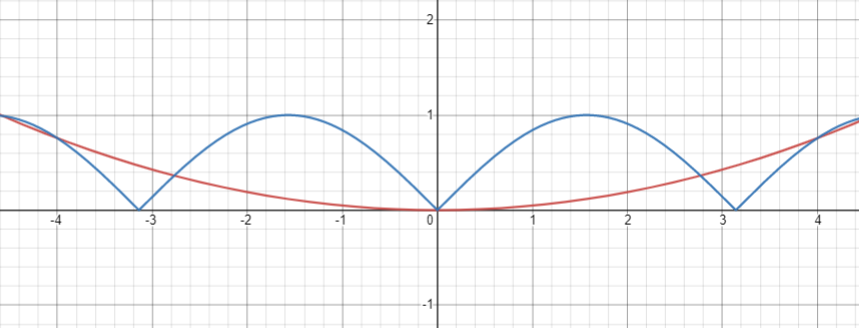
\includegraphics[scale=0.5]{wielomian2.PNG} \par
\vspace{3mm}
\hfil{Rysunek 1: Wykres funkcji $w_{2}(x)$} \par 

\vspace{5mm}
Analogicznie rozwiązanie dla wielomianu 5 stopnia:

\[w_{5}(x)=-4.517509\cdot 10^{-20}\cdot x^{5}+0.0010554x^{4}-0.0149577x^{2}+2.7755575615628\cdot 10^{-17}\cdot x+0.726141\]

\hfil
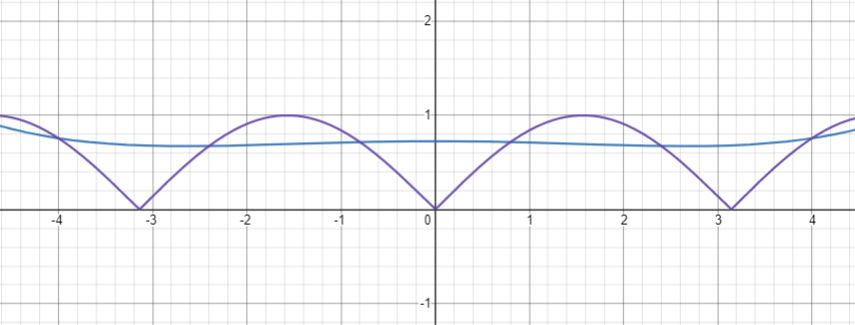
\includegraphics[scale=0.5]{wielomian5.PNG} \par
\vspace{3mm}
\hfil{Rysunek 2: Wykres funkcji $w_{5}(x)$} \par

\vspace{5mm}
Rozwiazanie dla wielomianu 10 stopnia:

\begin{multline*}
w_{10}(x) = 0.000313736x^{10} + 2.1684\cdot 10^{-19} x^{9} - 0.011196x^{8} - 6.93889\cdot 10^{-18} \cdot x^{7} + 0.138964 x^{6}\\ 
+ 5.55112\cdot 10^{-17}\cdot x^{5}-0.735417x^{4} - 1.11022\cdot 10^{-16} x^{3} + 1.53694 x^{2} - 1.11022\cdot 10^{-16} x
\end{multline*}

\hfil
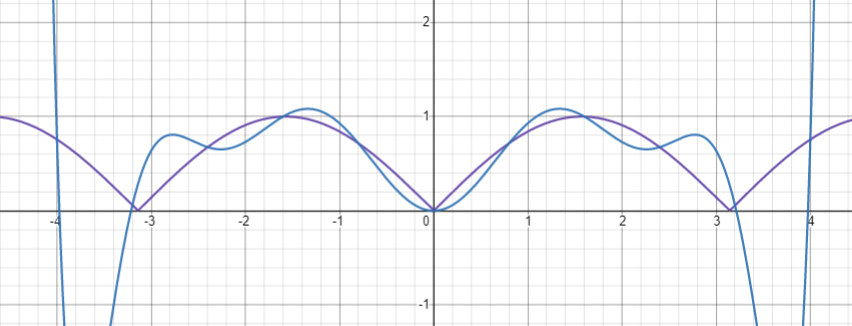
\includegraphics[scale=0.5]{wielomian10.PNG} \par
\vspace{3mm}
\hfil{Rysunek 3: Wykres funkcji $w_{10}(x)$} \par

\vspace{5mm}

\textbf{Wnioski:} \newline  
Wielomiany Lagrange'a 2 oraz 5 stopnia słabo przybliżają kształt funkcji $\left | \sin x \right |$. Ilość węzłów interpolacji jest zbyt mała. W przypadku wielomianu 5 stopnia, funkcja nie posiada miejsca zerowego, ze wzgledu na brak punktu o odciętej 0.\newline
Wielomian 10 stopnia w obszarze [-3,3] dosyć dobrze przybliża zadaną funkcję. Poza obszarem [-3,3] widać duże rozbieżności, jakość interpolacji jest zła. Jest to wynikiem efektu Rungego, który występuje w przypadku symetrycznego rozkładu węzłów interpolacji. Aby wyeliminować efekt Rungego należałoby zmienić rozkład węzłów interpolacji, gęściej umieszczając je na końcach przedziału.

\section{Bibliografia}

\begin{enumerate}
  \item \url{https://pl.wikipedia.org/wiki/Efekt_Rungego}
  \item \url{http://www.is.umk.pl/~kg/zajecia/MetNum2.pdf}
\end{enumerate}

\end{document}
